%####################################################################
%    Copyright @ 2007-2017 Andreas Frie� (Friess)
%    Permission is granted to copy, distribute and/or modify this document
%    under the terms of the GNU Free Documentation License, Version 1.2
%    or any later version published by the Free Software Foundation;
%    with no Invariant Sections, no Front-Cover Texts, and no Back-Cover Texts.
%    A copy of the license is included in the section entitled ``GNU
%    Free Documentation License''.
%%####################################################################
% Created: 24.05.2017
%%####################################################################
% !!!!! Copyrighted Text !!!!!! from
% https://msdn.microsoft.com/de-de/library/windows/desktop/dd375470(v=vs.85).aspx
%%####################################################################
This article describes the major components of DirectShow. It is intended as an introduction for application developers and for developers writing custom DirectShow filters. Application developers can usually ignore many of the low-level details of DirectShow. However, it is still a good idea to read this section, to have a general understanding of the DirectShow architecture.

\subsection{About DirectShow Filters}
DirectShow uses a modular architecture, where each stage of processing is done by a COM object called a filter. DirectShow provides a set of standard filters for applications to use, and developers can write their own custom filters that extend the functionality of DirectShow. To illustrate, here are the steps needed to play an AVI video file, along with the filters that perform each step:
\begin{itemize}
	\item Read the raw data from the file as a byte stream (File Source filter).
	\item Examine the AVI headers, and parse the byte stream into separate video frames and audio samples (AVI Splitter filter).
	\item Decode the video frames (various decoder filters, depending on the compression format).
	\item Draw the video frames (Video Renderer filter).
	\item Send the audio samples to the sound card (Default DirectSound Device filter).
\end{itemize}
These filters are shown in the following diagram \ref{fig:ic420231}.
\begin{figure}[!h]
	\centering
	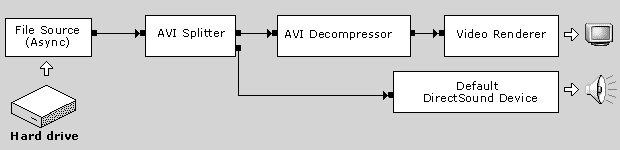
\includegraphics[width=0.7\linewidth]{ms_pic/IC420231}
	\caption{Filter Graph for playback}
	\label{fig:ic420231}
\end{figure}
Filter graph for playing back an AVI file with compressed video
As the diagram shows, each filter is connected to one or more other filters. The connection points are also COM objects, called \textit{pins}. Filters use pins to move data from one filter the next. The arrows in the diagram show the direction in which the data travels. In DirectShow, a set of filters is called a \textit{filter graph}.
\\Filters have three possible states: running, stopped, and paused. When a filter is running, it processes media data. When it is stopped, it stops processing data. The paused state is used to cue data before running; the section Data Flow in the Filter Graph describes this concept in more detail. With very rare exceptions, state changes are coordinated throughout the entire filter graph; all the filters in the graph switch states in unison. Thus, the entire filter graph is also said to be running, stopped, or paused.
Filters can be grouped into several broad categories:
\begin{itemize}
	\item A source filter introduces data into the graph. The data might come from a file, a network, a camera, or anywhere else. Each source filter handles a different type of data source.
	\item A transform filter takes an input stream, processes the data, and creates an output stream. Encoders and decoders are examples of transform filters.
	\item Renderer filters sit at the end of the chain. They receive data and present it to the user. For example, a video renderer draws video frames on the display; an audio renderer sends audio data to the sound card; and a file-writer filter writes data to a file.
	\item A splitter filter splits an input stream into two or more outputs, typically parsing the input stream along the way. For example, the AVI Splitter parses a byte stream into separate video and audio streams.
	\item A mux filter takes multiple inputs and combines them into a single stream. For example, the AVI Mux performs the inverse operation of the AVI Splitter. It takes audio and video streams and produces an AVI-formatted byte stream.
\end{itemize}
The distinctions between these categories are not absolute. For example, the ASF Reader filter acts as both a source filter and a splitter filter.
//All DirectShow filters expose the IBaseFilter interface, and all pins expose the IPin interface. DirectShow also defines many other interfaces that support more specific functionality.

\subsection{About the Filter Graph Manager}\footnote{Quelle: \cite{502}}
The Filter Graph Manager is a COM object that controls the filters in a filter graph. It performs many functions, including the following:
\begin{itemize}
	\item Coordinating state changes among the filters.
	\item Establishing a reference clock.
	\item Communicating events back to the application.
	\item Providing methods for applications to build the filter graph.
\end{itemize}
Each of these functions is described briefly here. Details can be found elsewhere in the documentation.


\begin{description}
	\item[State changes] State changes within filters must occur in a particular order. Therefore, the application does not issue state-change commands directly to the filters. Instead, it gives a single command to the Filter Graph Manager, which distributes the command to each of the filters. Seeking works in a similar fashion: The application gives a seek command to the Filter Graph Manager, which distributes it to the filters.
  	\item[Reference clock] All of the filters in the graph use the same clock, called a reference clock. The reference clock ensures that all the streams are synchronized. The time at which a video frame or audio sample should be rendered is called the presentation time. The presentation time is measured relative to the reference clock. The Filter Graph Manager chooses a reference clock, usually either the clock on the sound card, or the system clock.
	\item[Graph events] The Filter Graph Manager uses an event queue to inform the application of events that occur in the filter graph. This mechanism is similar to a Windows message loop.
	\item[Graph-building methods] The Filter Graph Manager provides methods for the application to add filters to the graph, connect filters to other filters, and disconnect filters.
\end{description}One function the Filter Graph Manager does not handle is moving data from one filter to the next. This is done by the filters themselves, through their pin connections. Processing always happens on a separate thread.
\begin{verse}
	\textbf{Note}\emph{  Filters are always free-threaded, reside in the same process as the Filter Graph Manager, and are loaded from in-process servers. Therefore, method calls are not marshaled between filters, or between filters and the Filter Graph Manager.}
\end{verse}

\subsection{About Media Types}
Because DirectShow is modular, it requires a way to describe the format of the data at each point in the filter graph. For example, consider AVI playback. Data enters the graph as a stream of RIFF chunks. These are parsed into video and audio streams. The video stream consists of video frames, which are probably compressed. After decoding, the video stream is a series of uncompressed bitmaps. The audio stream goes through a similar process.\\
Media Types: How DirectShow Represents Formats\\
The media type is a universal and extensible way to describe digital media formats. When two filters connect, they agree on a media type. The media type identifies what kind of data the upstream filter will deliver to the downstream filter, and the physical layout of the data. If two filters cannot agree on a media type, they will not connect.\\
For some applications, you will never have to worry about media types. In file playback, for example, DirectShow handles all of the details. Other kinds of applications may need to work directly with media types.\\
Media types are defined using the AM\_MEDIA\_TYPE structure. This structure contains the following information:
\begin{description}
	\item[Major type] The major type is a GUID that defines the overall category of the data. Major types include video, audio, unparsed byte stream, MIDI data, and so forth.
	\item[Subtype] The subtype is another GUID, which further defines the format. For example, within the video major type, there are subtypes for RGB-24, RGB-32, UYVY, and so forth. Within audio, there is PCM audio, MPEG-1 payload, and others. The subtype provides more information than the major type, but it does not define everything about the format. For example, video subtypes do not define the image size or the frame rate. These are defined by the format block, described below.
	\item[Format block] The format block is a block of data that describes the format in detail. The format block is allocated separately from the AM\_MEDIA\_TYPE structure. The pbFormat member of the AM\_MEDIA\_TYPE structure points to the format block.
\end{description}The pbFormat member is typed void* because the layout of the format block changes depending on the media type. For example, PCM audio uses a WAVEFORMATEX structure. Video uses various structures, including VIDEOINFOHEADER and VIDEOINFOHEADER2. The formattype member of the AM\_MEDIA\_TYPE structure is a GUID that specifies which structure is contained in the format block. Each format structure is assigned a GUID. The cbFormat member specifies the size of the format block. Always check these values before dereferencing the pbFormat pointer.\\
If the format block is filled in, then the major type and subtype contain redundant information. The major type and subtype, however, provide a convenient way to identify formats without a complete format block. For example, you can specify a generic 24-bit RGB format (MEDIASUBTYPE\_RGB24), without knowing all of the information required by the VIDEOINFOHEADER structure, such as image size and frame rate.\\
For example, a filter might use the following code to check a media type:

\begin{verbatim}
C++

HRESULT CheckMediaType(AM_MEDIA_TYPE *pmt)
{
    if (pmt == NULL) return E_POINTER;

    // Check the major type. We're looking for video.
    if (pmt->majortype != MEDIATYPE_Video)
    {
        return VFW_E_INVALIDMEDIATYPE;
    }

    // Check the subtype. We're looking for 24-bit RGB.
    if (pmt->subtype != MEDIASUBTYPE_RGB24)
    {
        return VFW_E_INVALIDMEDIATYPE;
    }

    // Check the format type and the size of the format block.
    if ((pmt->formattype == FORMAT_VideoInfo) &&
        (pmt->cbFormat >= sizeof(VIDEOINFOHEADER) &&
        (pmt->pbFormat != NULL))
    {
        // Now it's safe to coerce the format block pointer to the
        // correct structure, as defined by the formattype GUID.
        VIDEOINFOHEADER *pVIH = (VIDEOINFOHEADER*)pmt->pbFormat;

        // Examine pVIH (not shown). If it looks OK, return S_OK.
        return S_OK;
    }

    return VFW_E_INVALIDMEDIATYPE;
}
\end{verbatim}
The AM\_MEDIA\_TYPE structure also contains some optional fields. These can be used to provide additional information, but filters are not required to use them:
\begin{description}
	\item[lSampleSize] If this field is non-zero, it defines the size of each sample. If it is zero, it indicates that the sample size may change from sample to sample.
	\item[bFixedSizeSamples] If this Boolean flag is TRUE, it means the value in \textbf{lSampleSize} is valid. Otherwise, you should ignore \textbf{lSampleSize}.
	\item[bTemporalCompression] If this Boolean flag is FALSE, it means that all frames are key frames.
\end{description}

\subsection{About Media Samples and Allocators}
Filters deliver data across pin connections. Data moves from the output pin of one filter to the input pin of another filter. The most common way for the output pin to deliver the data is by calling the IMemInputPin::Receive method on the input, although a few other mechanisms exist as well.\\
Depending on the filter, memory for the media data can be allocated in various ways: on the heap, in a DirectDraw surface, using shared GDI memory, or using some other allocation mechanism. The object responsible for allocating the memory is called an allocator, which is a COM object that exposes the IMemAllocator interface.\\
When two pins connect, one of the pins must provide an allocator. DirectShow defines a sequence of method calls that is used to establish which pin provides the allocator. The pins also agree on the number of buffers that the allocator will create, and the size of the buffers.\\
Before streaming begins, the allocator creates a pool of buffers. During streaming, the upstream filter fills buffers with data and delivers them to the downstream filter. But the upstream filter does not give the downstream filter raw pointers to the buffers. Instead, it uses COM objects called media samples, which the allocator creates to manage the buffers. Media samples expose the IMediaSample interface. A media sample contains:
\begin{enumerate}
	\item a pointer to the underlying buffer
	\item a time stamp
	\item various flags
	\item optionally, a media type
\end{enumerate}
The time stamp defines the presentation time, which the renderer filter uses to schedule rendering. The flags indicate things like whether there was a break in the data since the previous sample. The media type provides a way for filters to change formats mid-stream. Usually, the sample has no media type, which indicates that the format has not changed since the previous sample.\\
While a filter is using a buffer, it holds reference count on the sample. The allocator uses the reference count to determine when it can re-use the buffer. This prevents a filter from overwriting a buffer that another filter is still using. A sample does not return to the allocator's pool of available samples until every filter has released it.\\
For more information, see the following topics:
\begin{itemize}
	\item The topic Samples and Allocators provides a more detailed description of how allocators work.
	\item The topic Data Flow in the Filter Graph gives a general overview of data flow in DirectShow.
\end{itemize}
The following topics are intended for developers who are writing their own custom filters:
\begin{itemize}
	\item Data Flow for Filter Developers
	\item Threads and Critical Sections
\end{itemize}

\subsection{How Hardware Devices Participate in the Filter Graph}
This article describes how DirectShow interacts with audio and video hardware.
\paragraph{Wrapper Filters}
All DirectShow filters are user mode software components. In order for a kernel mode hardware device, such as a video capture card, to join a DirectShow filter graph, the device must be represented as a user-mode filter. This function is performed by specialized \"wrapper\" filters provided with DirectShow. These filters include the Audio Capture filter, the VFW Capture filter, the TV Tuner filter, the TV Audio filter, and the Analog Video Crossbar filter. DirectShow also provides a filter called KsProxy, which can represent any type of Windows Driver Model (WDM) streaming device. Hardware vendors can extend KsProxy to support custom functionality, by providing a Ksproxy plug-in, which is a COM object aggregated by KsProxy.//
The wrapper filters expose COM interfaces that represent the capabilities of the device. The application uses these interfaces to pass information to and from the filter. The filter translates the COM method calls into device driver calls, passes that information to the driver in kernel mode, and then translates the result back to the application. The TV Tuner, TV Audio, Analog Video Crossbar, and KsProxy filters support custom driver properties through the IKsPropertySet interface. The VFW Capture filter and the Audio Capture filter are not extensible in this way.//
For application developers, wrapper filters enable the application to control devices just as they control any other DirectShow filter. No special programming is required; the details of communicating with the kernel-mode device are encapsulated within the filter.
\paragraph{Video for Windows Devices}
The VFW Capture filter supports earlier Video for Windows (VfW) capture cards. When a VfW card is present on the target system, it can be discovered and added to the filter graph using the DirectShow System Device Enumerator. For details, see Enumerating Devices and Filters.
\paragraph{Audio Capture and Mixing Devices (Sound Cards)}
Newer sound cards have input jacks for microphones and other types of devices. Typically these cards also have on-board mixing capabilities for controlling the volume, treble, and bass of each individual input. In DirectShow, the sound card's inputs and mixer are wrapped by the Audio Capture filter. Each sound card can be discovered with the System Device Enumerator. To view the sound cards in your system, run GraphEdit and select from the Audio Capture Sources category. Each filter in that category is a separate instance of the Audio Capture filter. (See Using GraphEdit.)
\paragraph{WDM Streaming Devices}
Newer hardware decoders and capture cards conform to the Windows Driver Model (WDM) specification. These devices have greater functionality than VfW devices. WDM video capture cards can support features that are not available under VfW, including the enumeration of capture formats, programmatic control of video parameters such as hue and brightness, programmatic input selection, and TV Tuner support.//
To support WDM streaming devices, DirectShow provides the KsProxy filter (ksproxy.ax). KsProxy has been called the \"Swiss Army Knife filter\" because it does so many different things. The number of pins on the filter, and the number of COM interfaces exposed by the filter, depend on the capabilities of the underlying driver. KsProxy does not appear in the filter graph under the name \"KsProxy.\" It always takes the friendly name of the device, which is found in the registry. To view the WDM devices on your system, run GraphEdit and select from the WDM Streaming categories. Even if you have only one WDM card on your system, that card might contain more than one device. Each device is represented as a separate filter, and each of these filters is actually KsProxy.//
An application uses the System Device Enumerator to find WDM device monikers on the system. KsProxy is instantiated by calling \textbf{BindToObject} on the moniker. Because KsProxy can represent all kinds of WDM devices, it must query the driver to determine which property sets the driver supports. Property sets are collections of data structures used by WDM drivers, and also by some user mode filters, such as MPEG-2 software decoders. KsProxy configures itself to expose the COM interfaces that correspond to those property sets. KsProxy translates the COM method calls into property sets and sends these to the driver. Hardware vendors can extend KsProxy by supplying plug-ins, which are vendor-specific interfaces that expose the special capabilities of a device. All these details are hidden from application. The application controls the device by way of KsProxy, in the same way as any other DirectShow filter.
\paragraph{Kernel Streaming}
WDM devices support kernel streaming, in which data is streamed entirely in kernel mode without ever switching to user mode. Switching between kernel mode and user mode is computationally expensive; kernel streaming allows for high bit rates without burdening the host CPU. WDM-based filters can use kernel streaming to pass multimedia data directly from one hardware device to another, either on the same card or on a different card, without copying the data into the system's main memory.//
From an application's point of view, it appears as if the data moves from one user-mode filter to the next. In reality, the data might never pass into user mode at all, but instead might be streamed directly from one kernel-mode device to another until it is rendered on the video graphics card. Some scenarios, such as capture to a file, require that the data pass from kernel mode to user mode at some point. However, this switch does not necessarily require the data to be copied to a new location in memory.//
Application developers generally do not need to be concerned with the details of kernel streaming, except as background information. See the Microsoft DDK for more detailed information about WDM, kernel streaming, KsProxy, and related topics.

